% -*- coding: utf-8 -*-

\chapter{序论}

\section{研究背景和意义}

移动互联网改变了大学生组织学习活动的方式。课程资料不再只来自教材，还包括课件、实验文档、网页链接、课堂笔记、课程群消息和复习清单等多种来源\cite{crompton2018use,sung2016effects}。这些资料常分散在备忘录、网盘、浏览器收藏夹和聊天记录中，导致学生在真正开始学习时需要反复寻找上下文。与此同时，任务拆解、番茄专注和学习复盘往往被放在不同应用里完成，数据之间缺少稳定连接，学习过程难以形成连续闭环。

现有工具在局部场景上已经取得了较好效果。待办类工具适合记录任务和截止时间，笔记类工具适合保存资料，番茄钟工具适合维持注意力，AI 助手适合生成摘要和行动建议\cite{kasneci2023chatgpt,kabudi2021ai}。但是这些工具通常存在三个问题：第一，资料与任务分离，资料沉淀后不一定能转化为可执行行动；第二，专注过程与任务上下文分离，番茄记录难以反向支撑复盘；第三，远程 AI 和云端服务依赖网络环境，一旦处于弱网或离线状态，核心学习流程容易被中断。

HarmonyOS 提供了 ArkTS、ArkUI、RDB、Preferences、AVPlayer、ArkWeb 和 Ability 等端侧能力，为构建本地优先的移动学习应用提供了基础\cite{harmonyos2024,zhang2023arkui}。本地优先思想强调核心数据和关键操作应优先保存在用户设备上，远程服务作为同步或增强能力存在\cite{kleppmann2019localfirst}。将该思想用于学习管理场景，可以使任务、资料、专注记录和复盘统计在离线状态下仍然可用，同时在网络可用时接入 AI 提炼和后端同步。

因此，本文设计并实现“知序”学习管理应用，目标是在 HarmonyOS 端侧建立“资料整理 - 任务分解 - 番茄执行 - 复盘反馈”的学习闭环。该研究具有实践意义：一方面，它能降低学生在多工具之间切换造成的认知成本；另一方面，它综合运用了移动端 UI、端侧数据库、原生能力调用、后端接口和数据库同步等课程知识，有助于验证移动应用开发课程的综合实践能力。

\section{本文主要工作}

本文围绕“知序”的设计与实现完成以下工作。

第一，分析大学生课程学习场景，明确资料、任务、专注和复盘四类核心对象，并确定系统必须满足离线可用、数据持久化、状态可解释和可扩展同步等要求。

第二，基于 HarmonyOS 与 ArkTS 构建移动端应用。客户端采用 MVVM 思路组织模型、视图和控制逻辑，使用 RDB 保存项目、任务、资料和番茄记录，使用 Preferences 保存计时器、登录态、AI 配置和同步配置。

第三，设计资料库与任务系统的闭环关系。用户可以保存笔记、链接、课件和文件引用；在 AI 服务可用时，系统可提炼资料摘要和要点，并进一步生成任务；任务完成后写入番茄记录，最终形成复盘统计。

第四，实现 Spring Boot + MyBatis 后端，提供用户登录、项目管理、任务管理、番茄记录、统计和同步接口。后端既支持 MySQL 运行环境，也保留 H2 作为快速演示和测试数据库。

第五，完成前后端功能测试、模拟器观察、构建脚本修复和论文模板编译验证，并根据测试结果优化快速添加入口、同步提示、白噪音资源加载和启动说明。

\section{论文组织结构}

本文共五章。第一章为序论，介绍研究背景、意义、主要工作和论文结构。第二章为工具选型，对开发语言、开发工具、前端框架、后端框架和数据库进行比较，并说明最终选择。第三章为系统设计，基于 MVVM 模式说明总体架构、模型层、视图层、控制层、网络部分和数据库设计。第四章为系统实现，说明主要功能的实现过程、运行效果、关键问题和解决方法。第五章为总结与展望，总结本文工作并说明后续可改进方向。

\chapter{工具选型}

\section{开发语言选型}

移动端开发语言主要可选 Java/Kotlin、Dart、JavaScript/TypeScript 和 ArkTS。Java/Kotlin 在 Android 生态中成熟，但不能直接体现 HarmonyOS 原生开发特性；Dart 适合 Flutter 跨平台开发，界面一致性较好，但在调用 HarmonyOS 端侧能力时需要额外适配；JavaScript/TypeScript 具有较强表达能力，但普通 TypeScript 缺少 HarmonyOS 声明式 UI 和系统能力约束；ArkTS 在 TypeScript 基础上面向 HarmonyOS 做了增强，能够直接使用 ArkUI、Ability、RDB 和系统服务接口。

综合课程要求和平台适配，本文客户端选择 ArkTS。该选择的优点是能够充分调用 HarmonyOS 原生能力，界面与状态绑定方式清晰，适合实现本地优先移动应用；不足是生态资料相对 Android 和 Web 更少，构建、签名和模拟器调试对开发环境要求更高。

后端语言主要可选 Java、Python 和 Node.js。Python 开发速度快，但在企业级分层和静态类型约束方面不如 Java；Node.js 适合高并发 I/O 和前后端同语言开发，但课程中数据库持久化和典型三层结构展示不如 Java 直观。Java 与 Spring Boot、MyBatis 结合成熟，适合构建 RESTful 接口和数据库访问层。因此，本文后端选择 Java。

\section{开发工具选型}

HarmonyOS 客户端开发工具主要可选 DevEco Studio 和通用代码编辑器。通用编辑器启动快、插件灵活，但缺少 HarmonyOS 模拟器、签名、HAP 打包和设备调试的一体化支持。DevEco Studio 集成 SDK、模拟器、Hvigor 构建、签名和 ArkTS 检查能力，是 HarmonyOS 应用开发的主要工具。因此，本文客户端开发选择 DevEco Studio。

后端开发工具可选 Eclipse、IntelliJ IDEA 和 Visual Studio Code。Eclipse 体积较轻，但 Spring Boot 项目的依赖管理和调试体验相对弱；Visual Studio Code 插件丰富，适合轻量编辑，但大型 Java 项目的重构和调试能力有限；IntelliJ IDEA 对 Maven、Spring Boot、MyBatis 和 Java 调试支持较完善。因此，后端开发更适合使用 IntelliJ IDEA 或 DevEco Studio 外部配合命令行 Maven。

在构建工具方面，前端采用 Hvigor，后端采用 Maven。Hvigor 是 HarmonyOS 工程默认构建工具，负责 ArkTS 编译、资源处理、HAP 打包和 APP 打包。Maven 负责后端依赖管理、测试和 JAR 打包，便于在不同机器上复现构建过程。

\section{前端框架选择}

HarmonyOS 前端可以选择 ArkUI 原生声明式开发，也可以通过 WebView 嵌入 H5 页面。H5 开发成本较低，图表和样式生态丰富，但端侧数据库、原生通知、文件选择、音频播放和 Ability 交互需要桥接，整体可靠性较低。ArkUI 能直接访问 HarmonyOS 端侧能力，状态驱动界面更新，适合构建与系统能力结合紧密的应用。

本文选择 ArkUI 作为主界面框架，并仅在复盘图表部分使用 ArkWeb 嵌入 Canvas 图表。这样可以兼顾原生交互和图表表达：任务、资料、专注和设置等高频操作由 ArkUI 实现，减少桥接成本；统计图表利用 Web 技术绘制，降低图形渲染实现复杂度。

\section{后端框架与数据库选择}

后端框架主要比较 Spring Boot、Express 和 Flask。Express 与 Flask 轻量灵活，适合快速原型，但在分层约定、数据库映射和工程规范方面需要自行补充。Spring Boot 提供成熟的依赖管理、配置体系和 REST 接口开发方式，与 MyBatis 结合后可清晰展示 Controller、Mapper 和 XML SQL 的分层结构。因此，本文后端选择 Spring Boot + MyBatis。

数据库方面，移动端使用 HarmonyOS RDB。它是端侧关系型数据库，适合保存任务、资料、番茄记录等结构化数据。后端数据库提供 MySQL 和 H2 两种运行方式。MySQL 适合正式演示服务器和课程要求中的关系型数据库展示；H2 文件数据库适合快速测试和无需额外安装数据库的场景。为满足演示稳定性，系统保留两种配置：默认启动脚本支持 MySQL，测试时可通过参数切换到 H2。

\chapter{系统设计}

\section{总体设计}

“知序”采用 MVVM 开发模式，将应用程序分为模型、视图、控制三大部分。模型部分负责描述业务对象和持久化结构，包括项目、任务、资料、番茄记录、设置和用户登录信息。视图部分负责页面展示和用户交互，包括今日、任务、资料、专注、复盘、我的、设置和同步等界面。控制部分负责连接视图与模型，处理用户操作、状态刷新、数据写入、AI 请求、后端同步和原生能力调用。

采用 MVVM 模式的优点在于：第一，页面不直接拼接数据库语句，降低界面和数据层耦合；第二，状态变化可以集中通过 Store 和服务层管理，减少不同页面之间的数据不一致；第三，后续增加后端同步、AI 提炼或新页面时，可以在服务层扩展能力，而不破坏已有视图结构。系统总体架构如图 \ref{fig:architecture} 所示。

\begin{figure}[htbp]
\centering
\begin{tikzpicture}[
  layer/.style={rectangle, draw, minimum width=9.4cm, minimum height=0.7cm, align=center, font=\small},
  arrow/.style={->, thick}
]
  \node[layer, fill=blue!10] (view) at (0, 2.8) {视图层：今日、任务、资料、专注、复盘、我的};
  \node[layer, fill=green!10] (control) at (0, 1.8) {控制层：FocusStore、设置服务、AI 服务、同步服务};
  \node[layer, fill=yellow!10] (model) at (0, 0.8) {模型层：Project、Task、Resource、Pomodoro、Settings};
  \node[layer, fill=orange!10] (local) at (0, -0.2) {端侧存储：RDB + Preferences};
  \node[layer, fill=red!10] (remote) at (0, -1.2) {扩展服务：Spring Boot 后端、远程 AI、ArkWeb 图表};
  \draw[arrow] (view) -- (control);
  \draw[arrow] (control) -- (model);
  \draw[arrow] (model) -- (local);
  \draw[arrow] (control) -- (remote);
\end{tikzpicture}
\caption{系统总体架构}
\label{fig:architecture}
\end{figure}

\section{模型部分设计}

模型部分围绕四类核心实体展开。项目用于组织课程或学习主题，包含名称、颜色和图标等信息。任务用于承载具体行动，包含标题、备注、所属项目、优先级、截止时间、状态、番茄数量、标签和子任务等信息。资料用于保存学习素材，包含标题、类型、正文摘录、摘要、要点、关联任务和复习时间。番茄记录用于描述一次专注过程，包含任务标识、开始时间、持续时长、是否完成和中断原因。

为了保证离线可用，模型数据首先写入端侧 RDB。任务状态采用待办、完成、删除三态设计，其中删除为软删除，不直接物理移除数据。资料状态分为活跃和归档，便于用户整理长期资料。标签、子任务和资料要点属于半结构化内容，在 ArkTS 中表现为数组，在数据库中以 JSON 字符串保存，以减少表结构复杂度。

设置类数据不适合放入业务表，因此使用 Preferences 保存。例如专注时长、白噪音类型、AI 接口地址、AI 模型、登录态、同步服务器地址等运行时配置分别存储在不同命名空间中。这样可以避免业务数据与配置数据相互污染，也便于后续清理或迁移。

\section{视图部分设计}

视图部分以底部标签页组织核心功能。今日页作为学习工作台，展示当日进度、快速添加任务和待办列表；任务页负责搜索、筛选、完成、删除和恢复任务；资料页负责资料录入、文件引用、资料筛选、AI 提炼和生成任务；专注页负责番茄计时、白噪音播放、中断记录和完成记录；复盘页展示本周专注时间、完成数量、项目分布和学习连续性；我的页整合复盘统计、资料库、云同步和设置入口。

界面设计遵循移动端高频操作优先原则。快速添加任务同时出现在今日页和任务页，减少用户为了添加任务而切换页面的成本。云同步页在未登录状态下明确提示模拟器与真机的服务器地址填写方式，避免用户把模拟器地址误用于真机。设置页将专注时长、白噪音和 AI 配置放在同一入口，保证影响专注体验的选项集中管理。

\section{控制部分设计}

控制部分以 FocusStore 和多个服务类为核心。FocusStore 作为页面状态门面，负责读取和刷新任务、项目、资料和番茄记录。页面在用户操作后调用 Store 或服务层方法，方法完成本地写入后刷新 Store，再同步到页面状态。该流程避免页面直接操作数据库，也减少多个页面状态不一致的问题。

设置服务负责读写 Preferences，并在用户修改专注时长或白噪音时立即保存。AI 服务负责保存模型配置、发起远程请求、解析响应并返回结构化建议。同步服务负责后端登录、拉取服务器数据、上推本地数据和更新同步时间。原生能力服务负责通知、后台保护和 AVPlayer 音频播放。

控制部分的关键原则是核心流程不依赖远程服务。任务新增、资料保存、番茄记录和复盘统计均在本地完成；AI 和后端只作为增强能力。如果远程 AI 未配置，系统只显示状态提示，不生成伪造结果；如果后端不可用，用户仍可继续使用本地学习闭环。

\section{网络与数据库设计}

网络部分分为 AI 请求和后端同步两类。AI 请求兼容常见 Chat Completions 风格接口，客户端保存 endpoint、model 和 apiKey。请求失败、密钥缺失或响应格式异常时，服务层返回明确错误状态，视图层向用户展示提示。后端同步采用 RESTful 接口，主要包括用户登录、项目接口、任务接口、番茄接口、统计接口、同步拉取和同步上推。

后端数据库包含 users、projects、tasks 和 pomodoros 四类主要表。users 保存用户账号信息；projects 保存项目名称、颜色、图标和更新时间；tasks 保存任务标题、备注、优先级、状态、截止时间、标签 JSON、子任务 JSON 和更新时间；pomodoros 保存番茄开始时间、持续时长、完成状态、中断原因和客户端请求标识。客户端请求标识用于降低重复提交导致的重复记录风险。

客户端和后端数据库并不是简单替代关系。客户端 RDB 是移动端运行的可信数据源，后端数据库是同步和备份目标。这样设计可以保证应用在没有后端时仍能运行，同时在需要跨设备或课程全栈展示时具备服务器扩展能力。

\section{本章小结}

本章从总体架构、模型、视图、控制、网络和数据库角度说明了“知序”的系统设计。系统以 MVVM 模式降低界面、业务和数据之间的耦合，以本地优先思想保证离线可用，以后端同步和 AI 服务提供可选增强能力。

\chapter{系统实现}

\section{工程结构与运行环境}

系统由 HarmonyOS 前端和 Spring Boot 后端组成。前端工程位于 entry 目录，主要代码集中在 pages、models、services、repository 和 utils 等模块中。pages 负责页面与组件，models 保存业务模型，services 封装数据库、设置、AI、同步、音频和原生能力，repository 处理登录相关数据，utils 保存格式化和设计常量。

后端工程位于 focus-server 目录，采用 Controller、Entity、Mapper、DTO 和 XML SQL 的结构组织。Controller 负责接收 HTTP 请求，Mapper 负责数据库访问，DTO 负责请求和响应数据传输。后端资源目录中同时提供 H2 和 MySQL 配置，便于在演示和测试之间切换。

运行环境方面，前端使用 DevEco Studio、HarmonyOS SDK 和 Hvigor 构建；后端使用项目自带 JDK 21 和 Maven 构建。为解决不同机器 Java 环境不一致的问题，项目提供后端环境脚本和前端构建脚本：后端脚本设置本地 JDK/Maven；前端构建脚本强制使用 DevEco Studio 自带 JBR，避免系统 Java 注册表异常影响 PackageApp。

\section{主要功能实现}

今日页实现了学习状态概览和快速添加任务。快速添加入口会把任务写入默认项目，并设置为较高优先级，写入成功后刷新任务列表。该入口同时出现在今日页和任务页，能够覆盖用户最常见的“想到一个任务立即记录”的场景。

任务管理实现了搜索、项目筛选、优先级筛选、完成切换、软删除和恢复。任务完成时更新状态和完成时间；删除时进入回收站而不是直接移除；恢复时重新回到待办列表。这种三态设计既提升误操作容错，也为后端同步保留删除语义。

资料库实现了手动资料录入和文件引用保存。用户可以保存笔记、网页链接、课件说明、PDF 摘录或本地文件 URI。系统只保存文件引用和用户备注，不直接复制大文件或解析文档全文，从而降低移动端权限和存储复杂度。资料被选中后，可以在 AI 配置可用时进行摘要和要点提炼，并将建议转换为任务。

专注模块实现了番茄计时、完成记录、中断记录和白噪音播放。用户开始专注时，系统根据设置启动计时器和环境音；完成或中断时停止音频并写入番茄记录。白噪音使用 rawfile 中的本地 MP3 文件，通过 AVPlayer 循环播放，避免依赖网络音频资源。

复盘模块根据本地任务和番茄记录计算统计数据，包括完成番茄数、专注分钟数、连续学习天数和周统计趋势。图表部分通过 ArkWeb 加载本地 HTML，并用 Canvas 绘制统计结果。云同步模块提供服务器地址、账号密码、登录和双向同步入口，登录成功后可执行先拉取后上推的数据同步流程。

\section{运行效果}

图 \ref{fig:today} 展示了今日页运行效果。页面上方呈现学习概览，中部提供快速添加任务入口，下方展示今日待办任务。该页面承担应用首页职责，使用户进入应用后可以直接判断当前任务状态并开始下一步行动。

\begin{figure}[htbp]
\centering
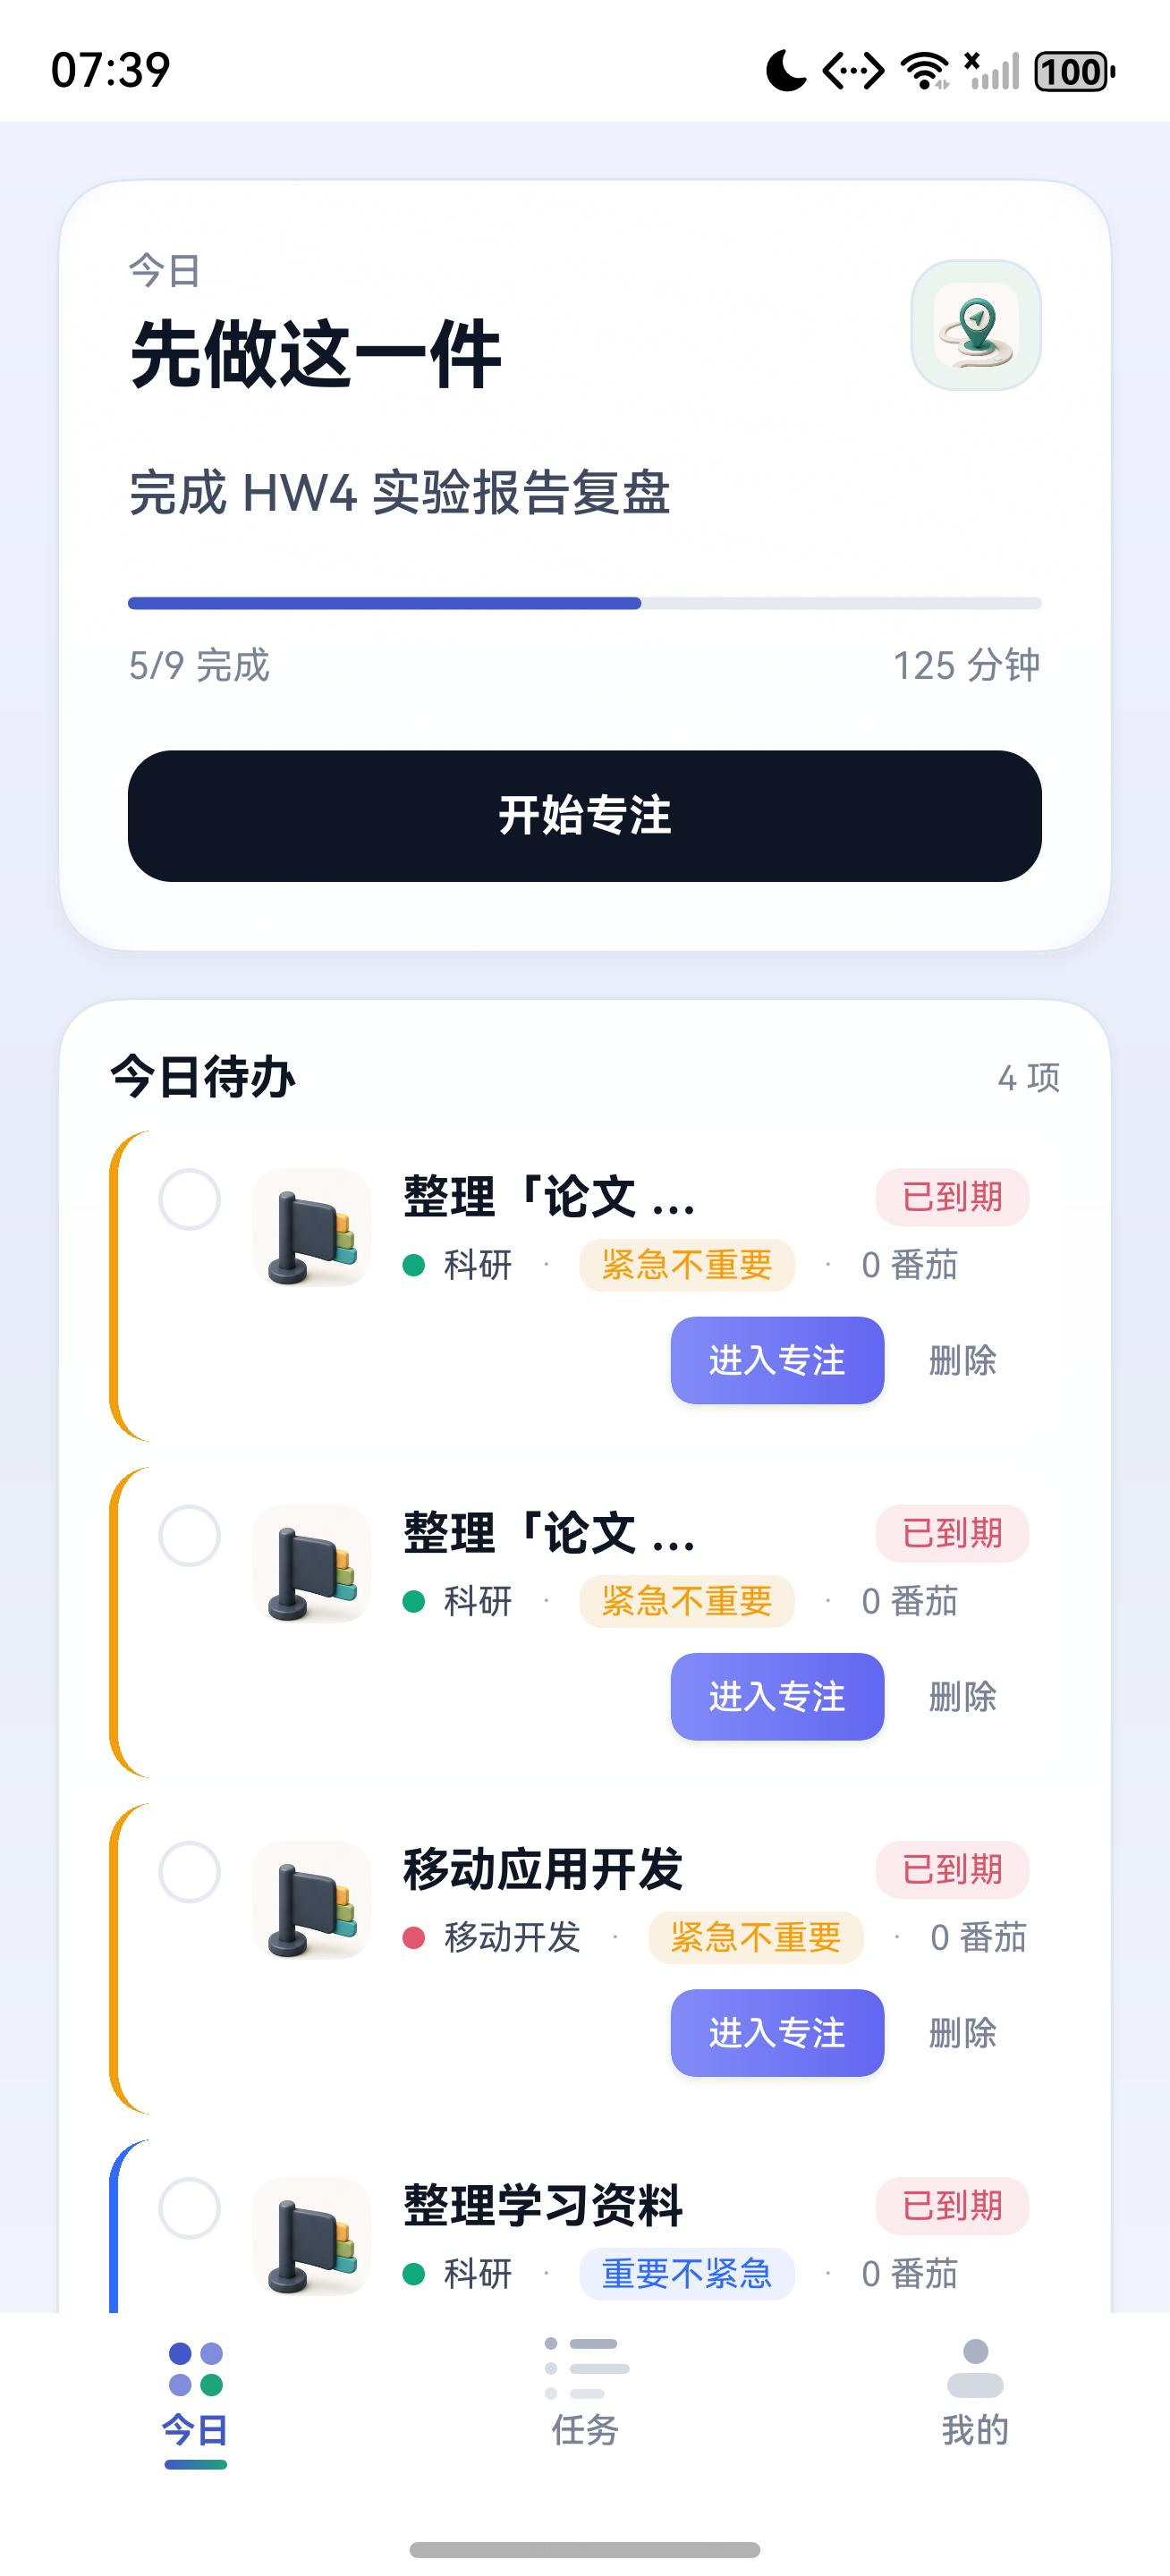
\includegraphics[width=0.42\textwidth]{figures/app-today.jpeg}
\caption{今日页运行效果}
\label{fig:today}
\end{figure}

图 \ref{fig:tasks} 展示了任务页运行效果。任务页提供任务列表、筛选条件和任务操作入口，适合集中处理课程任务、实验任务和复习任务。

\begin{figure}[htbp]
\centering
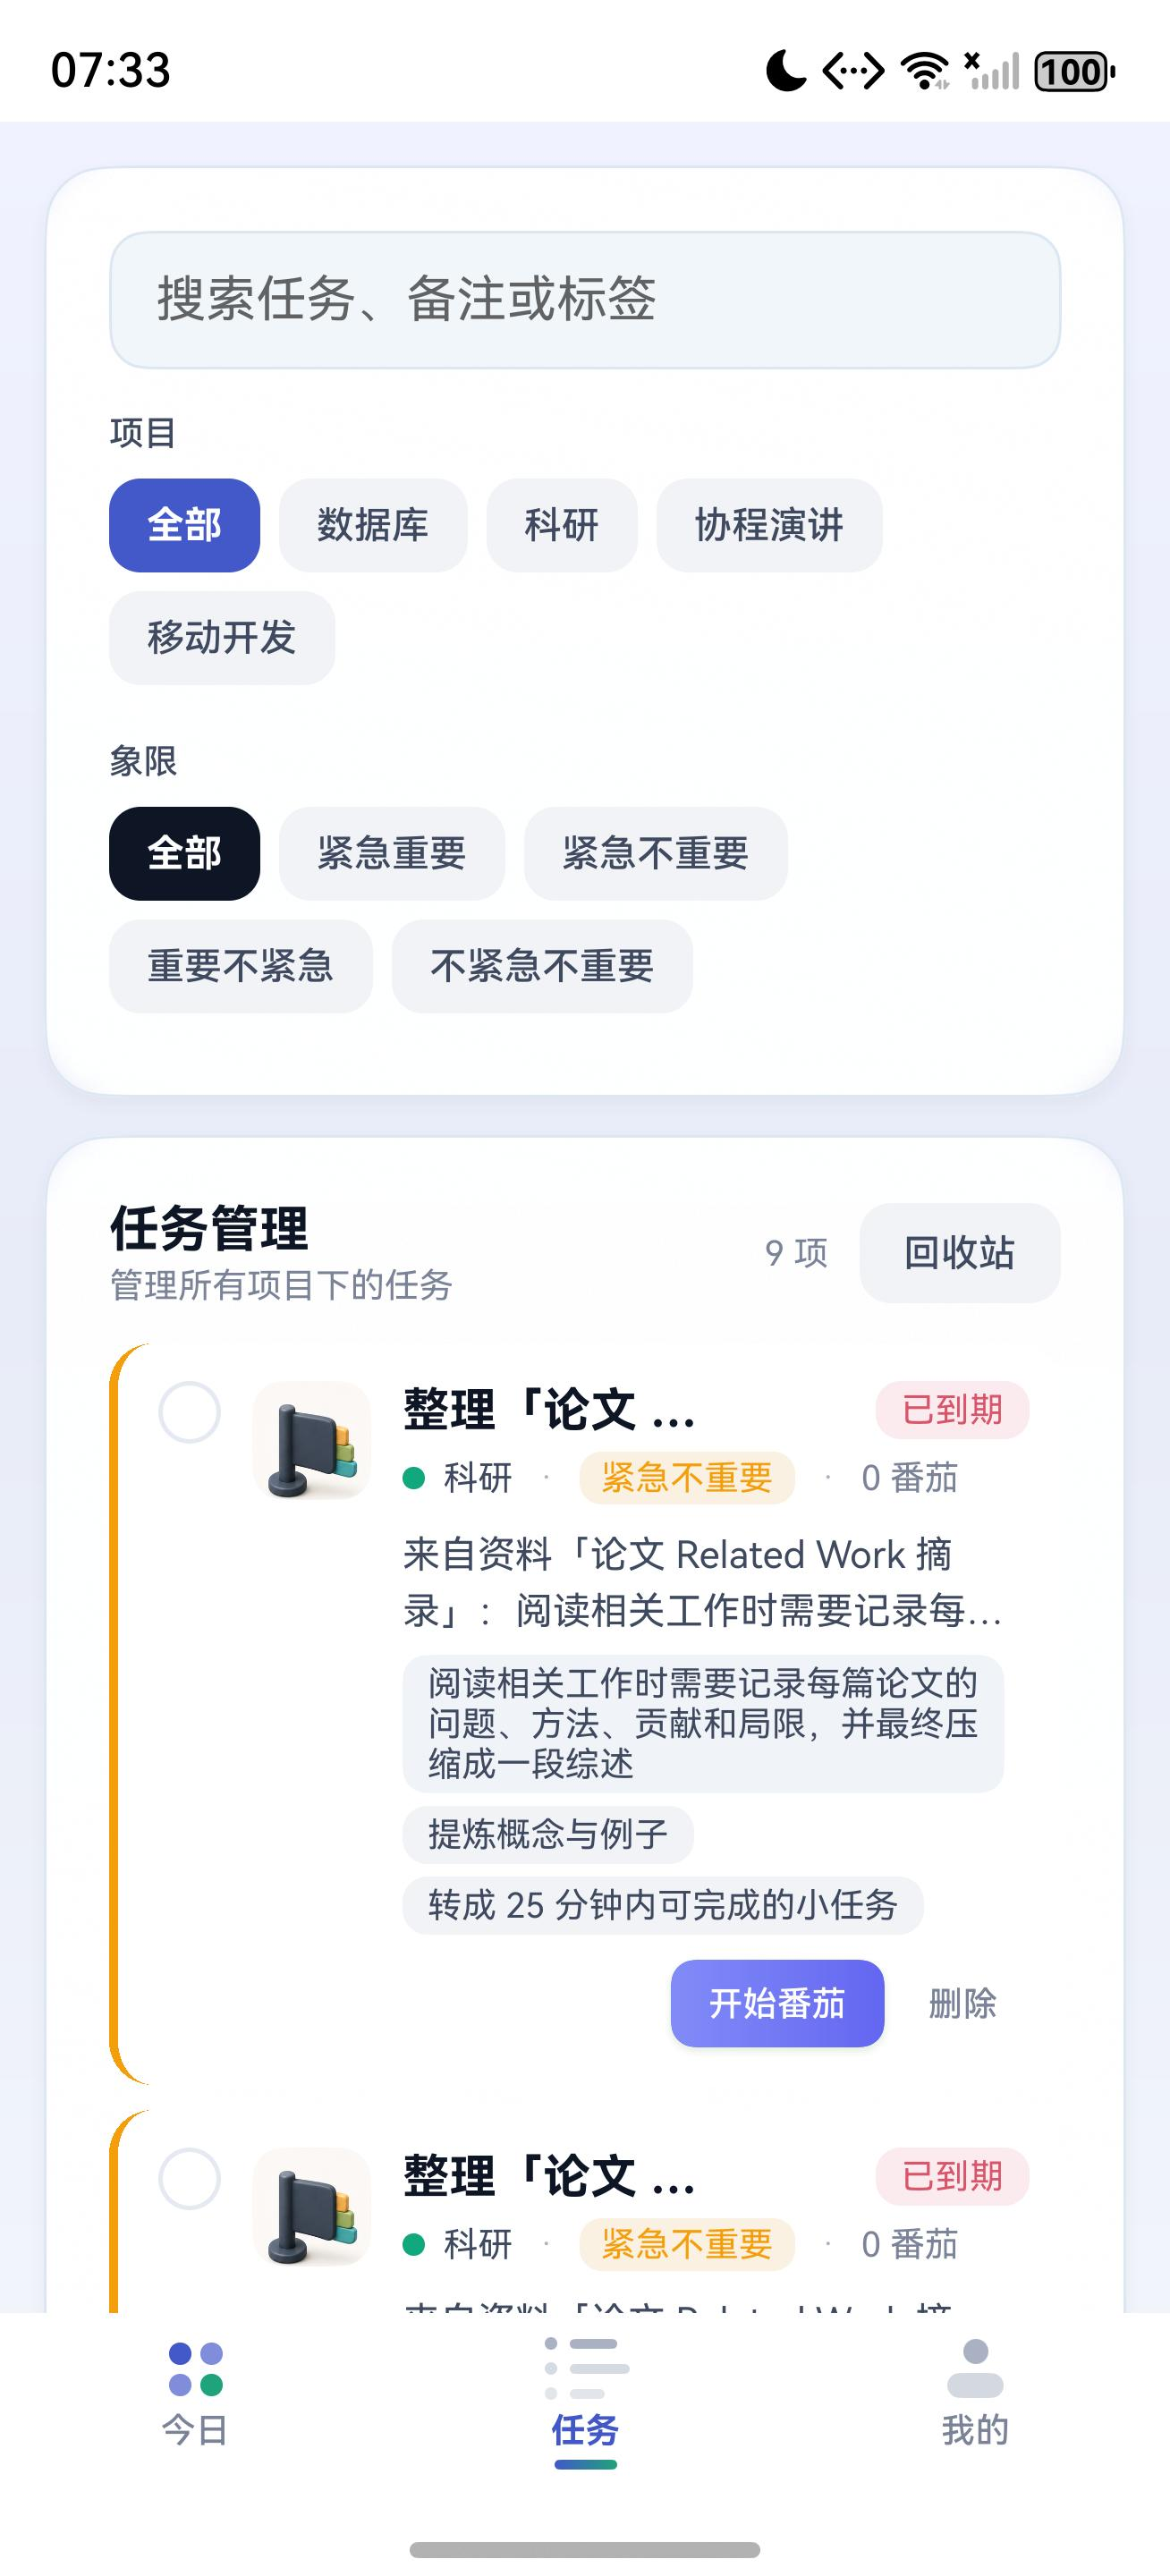
\includegraphics[width=0.42\textwidth]{figures/app-tasks.jpeg}
\caption{任务页运行效果}
\label{fig:tasks}
\end{figure}

图 \ref{fig:profile} 展示了我的页运行效果。该页面集中放置复盘统计、学习资料库、云同步和设置入口，适合作为高级功能与系统配置的统一入口。

\begin{figure}[htbp]
\centering
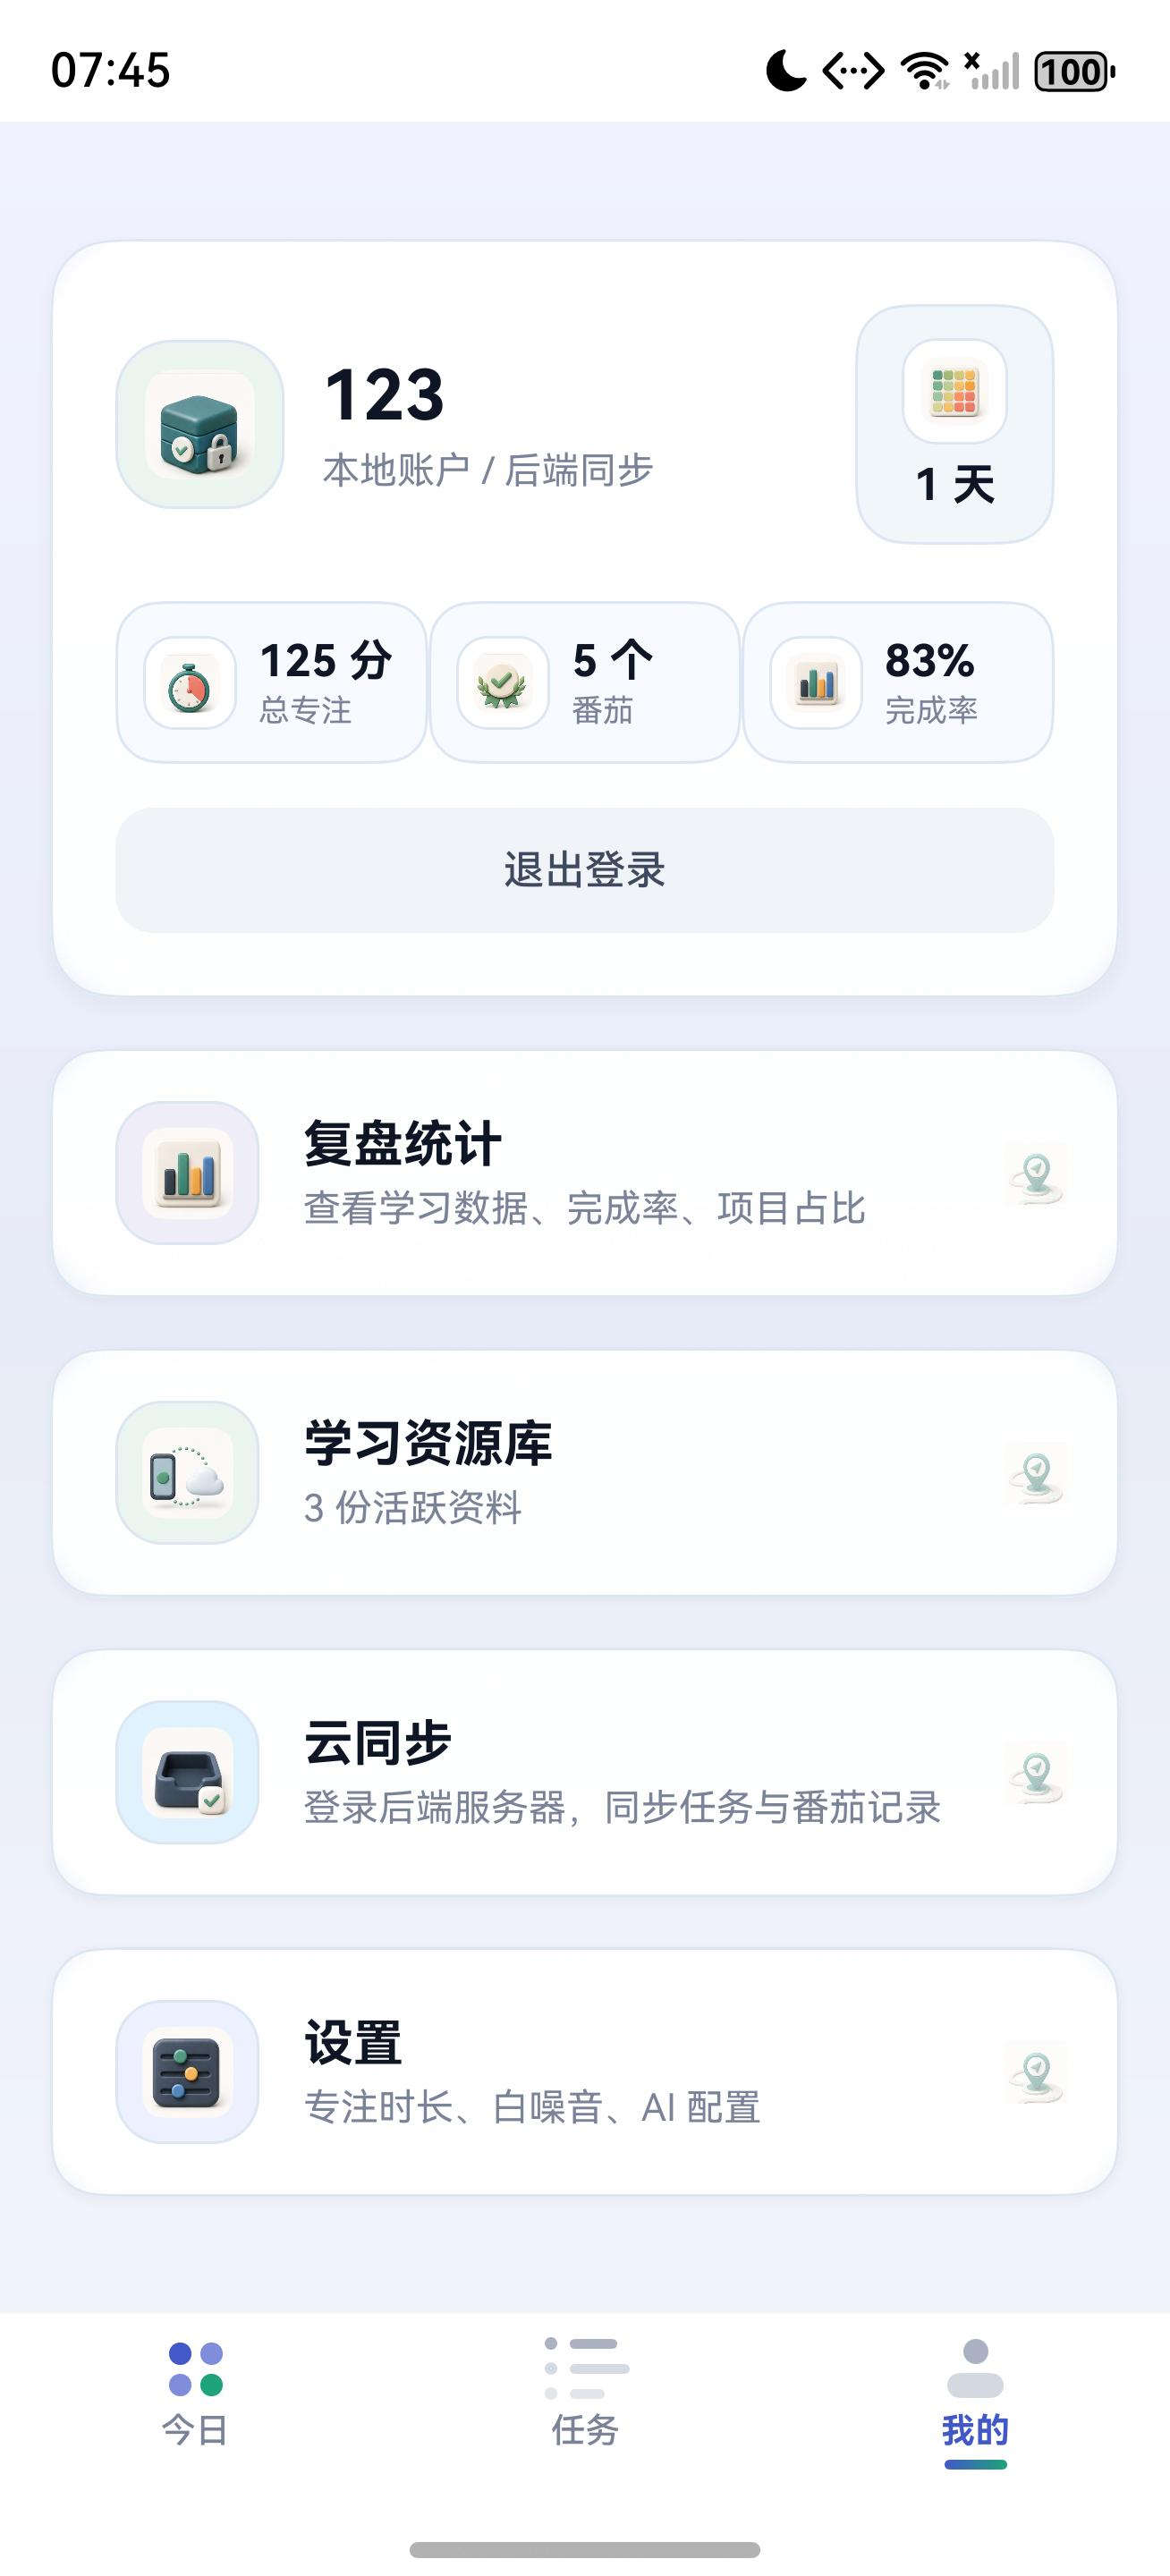
\includegraphics[width=0.42\textwidth]{figures/app-profile.jpeg}
\caption{我的页运行效果}
\label{fig:profile}
\end{figure}

\section{关键问题与解决方法}

实现过程中遇到的第一个问题是前端最终 PackageApp 被系统 Java 注册表异常阻塞。ArkTS 编译和 PackageHap 可以通过，但 PackageApp 阶段调用到系统 Java 时会受到错误注册表配置影响。解决方法是增加专门的前端构建脚本，在脚本中设置 JAVA\_HOME 和 PATH，强制使用 DevEco Studio 自带 JBR，并移除 Oracle javapath 的干扰。这样可以绕过系统 Java 注册表问题，使完整 APP 打包流程可复现。

第二个问题是后端环境脚本存在语法错误，导致测试启动前就被脚本拦截。解决方法是重写脚本，使其只负责设置项目自带 JDK 和 Maven，并在执行后输出 Java 与 Maven 版本。后端真正启动由 start-backend 脚本负责，从而区分“配置环境”和“启动服务”两个职责。

第三个问题是白噪音资源加载失败。原始音频资源使用中文文件名，在构建和资源访问过程中容易出现路径匹配问题。解决方法是将 rawfile 音频文件统一改为 ASCII 文件名，例如 outdoor.mp3、ocean.mp3 和 cricket.mp3，并在播放服务中维护枚举到文件名的映射。这样可以减少资源路径在不同工具链中的编码风险。

第四个问题是默认项目硬编码。早期快速添加和资料保存逻辑依赖固定项目 id，一旦种子数据或数据库状态变化，就可能写入错误项目。解决方法是改为按项目名称查找“移动开发”，找不到时使用第一个项目作为兜底，并让资料项目选择器的初始高亮与实际保存逻辑一致。

第五个问题是后端数据库选择带来的演示差异。MySQL 适合正式演示，但需要提前创建 focus\_db 并导入初始化脚本；H2 启动成本低，适合自动化测试和课堂快速演示。项目保留两种配置，并在文档中说明默认 MySQL 与 H2 参数切换方式，以免测试阶段因本机未安装 MySQL 而误判后端不可用。

\section{测试与验证}

后端接口测试覆盖项目、任务、番茄、统计和同步流程。使用 H2 模式启动后，可以完成登录 demo/secret、项目列表查询、任务创建与更新、番茄记录创建、统计查询、同步拉取和同步上推。该结果说明后端接口和数据库映射可以支撑移动端同步功能。

前端模拟器观察覆盖今日页、任务页、我的页、任务完成切换和白噪音播放。测试中任务完成状态能够影响今日进度，白噪音在专注时可以播放，说明本地状态刷新和 AVPlayer 调用有效。对 UI 的进一步检查发现，快速添加入口应同时出现在今日页和任务页，同步页应明确区分模拟器地址和真机局域网地址，这些问题已在实现中优化。

构建验证包括后端 Maven 测试、前端 HAP/APP 构建和论文 LaTeX 编译。后端脚本修复后可以使用项目自带 JDK/Maven 执行测试。前端构建脚本修复后可以通过 PackageApp。论文模板使用自动目录机制，目录由章节标题生成，而不是手工输入。

\section{本章小结}

本章说明了系统工程结构、核心功能实现、运行效果、关键问题和测试验证情况。实现结果表明，“知序”已经具备学习资料保存、任务管理、番茄专注、复盘统计和后端同步的基本闭环，并通过脚本和界面优化提升了项目演示稳定性。

\chapter{总结与展望}

\section{总结}

本文完成了基于 HarmonyOS 的本地优先学习管理应用“知序”的设计与实现。系统以 ArkTS 和 ArkUI 构建移动端界面，以 RDB 保存项目、任务、资料和番茄记录，以 Preferences 保存运行时配置，并按照 MVVM 模式组织模型、视图和控制逻辑。通过今日、任务、资料、专注、复盘和云同步等模块，系统将学习资料沉淀、任务执行、专注记录和复盘反馈连接为一个完整闭环。后端采用 Spring Boot 与 MyBatis 实现 RESTful 接口，并通过 MySQL/H2 支持正式演示和快速测试两种运行方式。测试结果表明，系统核心功能可以在离线状态下运行，后端可用时能够完成同步流程，整体满足课程项目对移动端开发、数据库设计、原生能力调用和全栈接口展示的要求。

\section{展望}

后续工作可以从四个方向继续完善。第一，增强资料处理能力，在文件引用基础上加入 PDF、DOCX、PPTX 正文解析和 OCR，使资料库能够处理更完整的学习材料。第二，提升同步能力，增加冲突解决策略、同步历史、失败重试和多设备状态提示，使后端同步更接近真实产品。第三，完善 AI 功能，加入结果缓存、提示词模板管理和更严格的结构化校验，降低外部服务波动对体验的影响。第四，继续优化前端体验，包括横屏和平板布局、无障碍适配、服务卡片真实数据接入、复盘图表交互和更细致的视觉层级，使应用从课程原型进一步接近可长期使用的学习工具。
